

\tikzset{every picture/.style={line width=0.3pt}} %set default line width to 0.75pt        

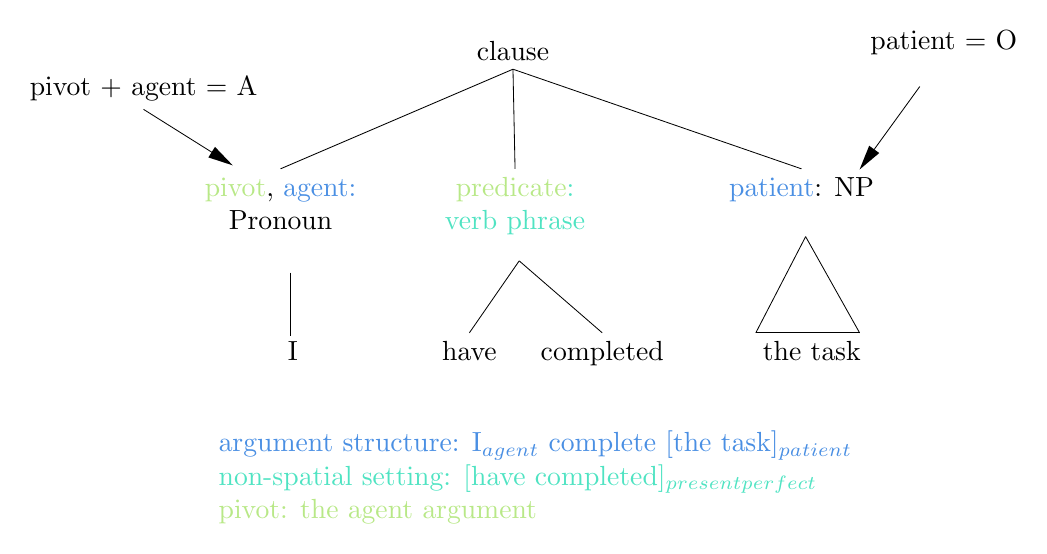
\begin{tikzpicture}[x=0.75pt,y=0.75pt,yscale=-1,xscale=1]
%uncomment if require: \path (0,390); %set diagram left start at 0, and has height of 390

%Straight Lines [id:da4161051988460063] 
\draw    (357,91.81) -- (245,139.81) ;
%Straight Lines [id:da36248311433047187] 
\draw    (360,184.15) -- (336,218.81) ;
%Straight Lines [id:da4439661314753782] 
\draw    (360,184.15) -- (400,218.81) ;
%Straight Lines [id:da36890954567869483] 
\draw    (474,218.81) -- (524,218.81) ;
%Straight Lines [id:da011342458373226894] 
\draw    (498,172.48) -- (474,218.81) ;
%Straight Lines [id:da5435200709744346] 
\draw    (498,172.48) -- (524,218.81) ;
%Straight Lines [id:da24568188379824396] 
\draw    (250,189.81) -- (250,220.48) ;
%Straight Lines [id:da3308532295080375] 
\draw    (357,91.81) -- (358,139.81) ;
%Straight Lines [id:da7487945318074942] 
\draw    (357,91.81) -- (496,139.81) ;
%Straight Lines [id:da4563709965960021] 
\draw    (179,111.15) -- (220.31,137.08) ;
\draw [shift={(222,138.15)}, rotate = 212.12] [fill={rgb, 255:red, 0; green, 0; blue, 0 }  ][line width=0.08]  [draw opacity=0] (12,-3) -- (0,0) -- (12,3) -- cycle    ;
%Straight Lines [id:da9447643488804027] 
\draw    (553,100.15) -- (525.17,138.53) ;
\draw [shift={(524,140.15)}, rotate = 305.94] [fill={rgb, 255:red, 0; green, 0; blue, 0 }  ][line width=0.08]  [draw opacity=0] (12,-3) -- (0,0) -- (12,3) -- cycle    ;

% Text Node
\draw (251,221.81) node [anchor=north] [inner sep=0.75pt]   [align=left] {I};
% Text Node
\draw (336,221.81) node [anchor=north] [inner sep=0.75pt]   [align=left] {have};
% Text Node
\draw (400,221.81) node [anchor=north] [inner sep=0.75pt]   [align=left] {completed};
% Text Node
\draw (501,221.81) node [anchor=north] [inner sep=0.75pt]   [align=left] {the task};
% Text Node
\draw (358,142.81) node [anchor=north] [inner sep=0.75pt]  [color={rgb, 255:red, 80; green, 227; blue, 194 }  ,opacity=1 ] [align=left] {\begin{minipage}[lt]{54.34pt}\setlength\topsep{0pt}
\begin{center}
\textcolor[rgb]{0.72,0.91,0.53}{predicate}:\\verb phrase
\end{center}

\end{minipage}};
% Text Node
\draw (496,142.81) node [anchor=north] [inner sep=0.75pt]   [align=left] {\textcolor[rgb]{0.29,0.56,0.89}{patient}: NP};
% Text Node
\draw (245,142.81) node [anchor=north] [inner sep=0.75pt]   [align=left] {\begin{minipage}[lt]{61.87pt}\setlength\topsep{0pt}
\begin{center}
\textcolor[rgb]{0.72,0.91,0.53}{pivot}, \textcolor[rgb]{0.29,0.56,0.89}{agent:} \\Pronoun
\end{center}

\end{minipage}};
% Text Node
\draw (357,88.81) node [anchor=south] [inner sep=0.75pt]   [align=left] {clause};
% Text Node
\draw (214,265) node [anchor=north west][inner sep=0.75pt]   [align=left] {\textcolor[rgb]{0.29,0.56,0.89}{argument structure: I$\displaystyle _{\text{agent}}$ complete [the task]$\displaystyle _{\text{patient}}$}\\\textcolor[rgb]{0.31,0.89,0.76}{non-spatial setting: [have completed]$\displaystyle _{\text{present perfect}}$}\\\textcolor[rgb]{0.72,0.91,0.53}{pivot: the agent argument }};
% Text Node
\draw (528,72) node [anchor=north west][inner sep=0.75pt]   [align=left] {patient = O};
% Text Node
\draw (179,108.15) node [anchor=south] [inner sep=0.75pt]   [align=left] {pivot + agent = A};


\end{tikzpicture}
